\documentclass{sig-alternate-05-2015}
\usepackage{amsmath}
\usepackage[T1]{fontenc}
\newcommand\numberthis{\addtocounter{equation}{1}\tag{\theequation}}
\usepackage{multirow}

\begin{document}

\author{Alun Meredith\vspace{-2ex}% Toggle commenting out the command
}
\title{Kalman Filtering and Lasso Regularisation \vspace{-2ex}% to see the effect
}
\maketitle

\vspace{-30mm}

\begin{abstract}
In this paper we consider the ability to model the noise of index movements after smoothing through econometric measures. Kalman smoothing and auto-regression are used to model the underlying trends of the Monthly S\&P 500 index and Lasso regularised linear regression to model the residuals. We find that using an order 10 Kalman smoother an $R^2$ of 0.33 can be obtained with a P value of 0.059. We also find that over time different econometric variables become relevant and during periods of low residuals none of these variables can be used to explain the residuals. 
\end{abstract}

\section{Noise Filtering}

\subsection{Auto-regressive models}

Auto-regression models the behaviour of stock price today as a function of the previous days plus some random noise:

\begin{equation}
y_{t} = \sum_{i=1}^{Order} \beta_i y_{t-i} + \epsilon_t
\end{equation}

It is natural to think of stock price as auto-regressive; today's price is yesterdays price + returns. Although it is not clear what order the function would take and a stationary form clearly over-simplifies, for example volatility (size of the noise term) is known to not be stationary. 

An auto-regression model can easily by computed by minimising least squares with the pseudo-inverse for a set of time lagged features, such as for Order = 3 below:

\begin{align}
\begin{bmatrix}
  x_1 & x_2 & x_3 \\ 
  x_2 & x_3 & x_4 \\ 
  \vdots & \vdots & \vdots \\ 
  x_{n-3} & x_{n-2} & x_{n-1} \\
\end{bmatrix}
\begin{bmatrix}
  \beta_1 \\ 
  \beta_2 \\ 
  \vdots \\ 
  \beta_{Order} \\ 
\end{bmatrix}
=
\begin{bmatrix}
  y_4 \\ 
  y_5 \\ 
  \vdots \\ 
  y_n \\ 
\end{bmatrix}
\end{align}

\subsection{Kalman Filtering}
Another method of filtering the noise of a signal is using Kalman filtering. This is a state based model with the advantage that it is updated iteratively. This means that upon receiving new data the model isn't recomputed but updated, a much more computationally efficient process which also benefits from localised modelling i.e. can capture changes to the underlying nature of the data.  

The state space model is defined as an underlying value $\theta$ following an order 1 autoregressive function and an observed stock price as $z$ which is the underlying value augmented by some noise. There are only two parameters which need to be defined; the noise of the observation $V$, estimated as the variance variance in residual from the AR model and the noise of the underlying value $W$ which is tuned empirically using cross validation and RMSE. 

\begin{align}
&z_t = \theta_t + v_t \qquad &v_t \sim N(0, V) \\
&\theta_t = \theta_{t-1} + \omega_t \qquad &\omega_t \sim N(0, W) \\
&\theta_0 \sim N(m_0, V)
\end{align}

This leads to the following set of iterative update equations:
\begin{align*}
\mathtt{Prediction} \\
\hat{\theta}_{t|t-1} = \hat{\theta}_{t|t-1} \\
P_{t|t-1} = P_{t-1|t-1} + W \\
\mathtt{Correction} \\
r_t = z_t - \hat{\theta}_{t|t-1} \\
S_t = P_{t|t-1} + V \\
K_t = P_{t|t-1}S_t^{-1} \\
\hat{\theta}_{t|t} = \hat{\theta}_{t|t-1} + K_tr_t \\
P_{t|t} = (1 - K_tH_t)P_{t|t-1}
\end{align*}

We simulate an autoregressive function to test the Kalman filtering: 

\begin{equation}
 Y = 0.7Y_{t-1} + 0.3Y_{t-2} + \eta \qquad \eta \sim N(1,0.1) \label{simulation}
\end{equation}

Figure \ref{fig:Weight_Estimation} shows how the Kalman filtering algorithm estimates the underlying weights of the autoregressive model. It shows that there is high variance initially but quickly gets close to the correct weights but doesn't converge to them. 

Figure \ref{fig:W_variation} shows the effect of the size of the evolution noise $W$. As the value decreases smoothing increases, this is due to a higher level of certainty $P$ for the current prediction and therefore less weight associated to the correction. 

\begin{figure}[ht]

				%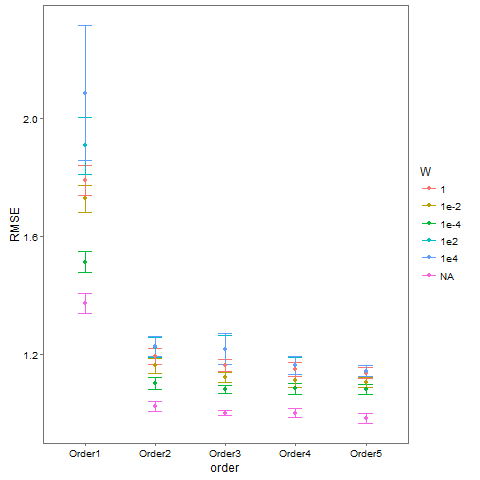
\includegraphics[width=\linewidth]{RMSE_order.png}
	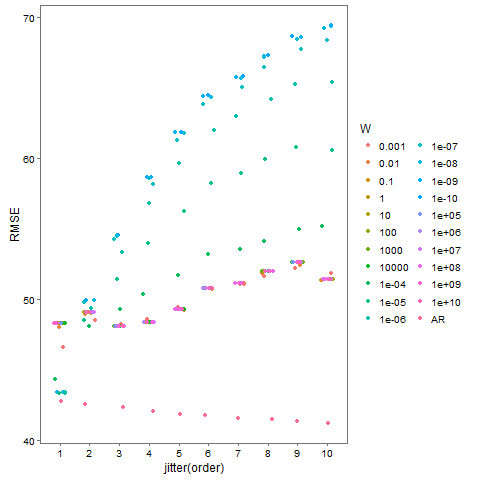
\includegraphics[width=\linewidth]{RMSE_order_real.png}
	\centering
	\caption{RMSE of Kalman smoothing and AutoRegression against Historic Data for a variety of orders and W values, x value is "jittered" with some random noise to show overlapping points}
			\label{fig:RMSE_real}

\end{figure}

\begin{figure}[ht]

	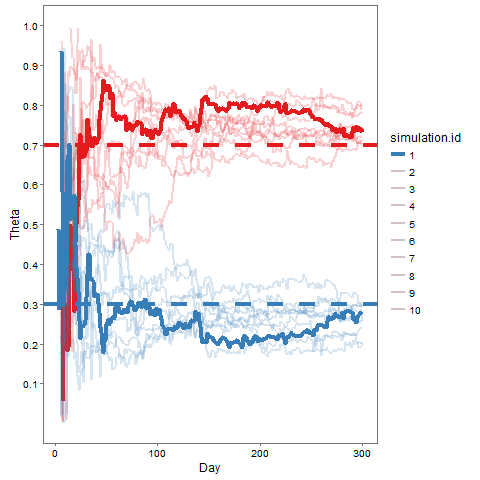
\includegraphics[width=0.7\linewidth]{Test_Weight_Estimation.png}
	\centering
	\caption{The prediction of underlying auto-regression weights from Kalman filtering over time for simulated data \eqref{simulation} (W = 1e-4)}
			\label{fig:Weight_Estimation}
			
	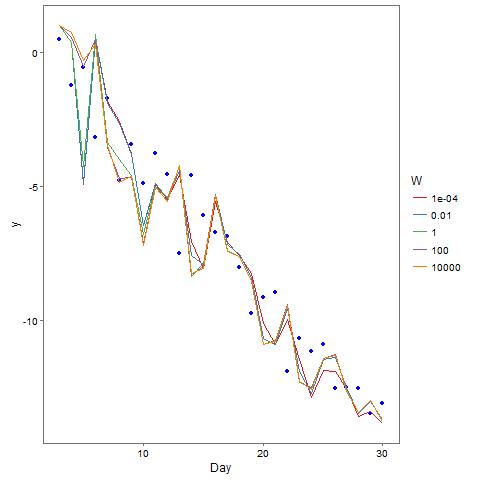
\includegraphics[width=0.7\linewidth]{W_variation.png}
	\centering
	\caption{The Kalman smoothing vs. observed values for a variety of W values for simulated data \eqref{simulation}}
			\label{fig:W_variation}
			
		
				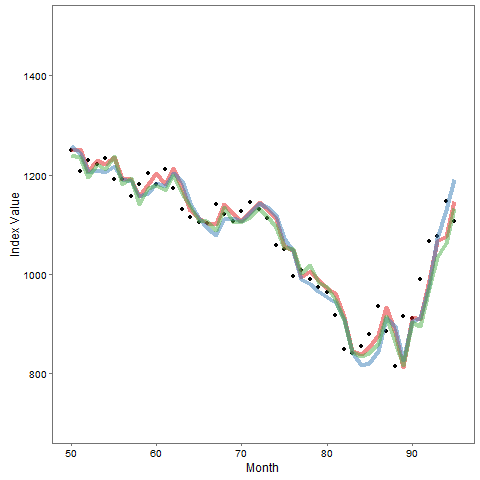
\includegraphics[width=0.7\linewidth]{DifferentModels.png}
	\centering
	\caption{Effects of smoothing for: \textbf{Kalman} Order 1, W 1e-7 (red), \textbf{Kalman} Order 5, W 1e5 (blue) and \textbf{Autoregression}, Order 3 (green). On a subset of the data (Months 50-100, chosen to give Kalman filters enough time to train and capture shifts in the direction of the data)}
			\label{fig:DifferentModels}
\end{figure}

\subsection{Filtering on S\&P 500}
The time series data used for the rest of this paper is the Monthly S\&P 500 index from 01-01-1889 to 01-01-2009. \footnote{Source: Yahoo finance}

The Kalman Filter is parametrised by its order and its evolution noise $W$, but these must be found empirically. Evaluating Kalman Smoothing and auto-regression (AR) on the S\&P data for a variety of orders and $W$ values fig. \ref{fig:RMSE_real} we see that the AR model performs better than Kalman Smoothing however the AR model uses the time-series as a training set whereas Kalman smoothing makes an unseen prediction at each timestep. 
For low orders of Kalman low W values perform best whereas for higher orders high W values perform best. This makes sense as if the order of the Kalman doesn't encapsulate the underlying order a low W value retains previous predictions more, keeping information from the previous timesteps in an emulation of a higher order process. Errors tend to increase for the higher order Kalman filters, this is likely due to over-fitting i.e. under-smoothing, as higher orders produce more complex models.  Finally we see that very low values of W converge together as do high values of W. These represent the points where the first term or W term dominates in the uncertainty update. I.e. the uncertainty of my prediction is either exactly equal to the previous uncertainty (for low W) or completely uncertain so assign no weight to my prediction (for high W).  

Based on the RMSE results of figure \ref{fig:RMSE_real}, 4 models were chosen to continue the analysis: the order = 3, AR model; order = 1, W = 1e-7 Kalman; order = 5, W = 1e5 Kalman and order = 10, W = 1e5 Kalman. Figure \ref{fig:DifferentModels} shows how these models fit a small window of the data.   

\clearpage
\section{Lasso Regularisation}
In this section we try to explain the residuals produced by the above models through Lasso regularised linear regression on econometric data. The variables used match those used by Mahler over the same timescale of the S\&P index \footnote{source: Federal Reserve Bank of St. Louis} \cite{mahler2009modeling}: 
\begin{itemize}
\item SP\_PE: S\&P 500 Price-to-Earnings Ratio 
\item CORP.PROFIT: Corporate Profits after tax
\item POPULATION: US Population
\item UNEMPLOYMENT: US Unemployment rate
\item INCOME: Disposable Personal Income
\item PMI: Purchasing Manager's Index
\item OILPRICE: Spot Oil Price, West Texas Intermediate
\end{itemize}

Lasso regularisation attempts to minimise the sum of the squared error with a Manhattan distance penalty term. This imposes a sparsity bias which is useful variable selection while improving generalisation. The Lagrangian form of lasso regularisation is given below:

\begin{align}
\min_\beta\left\lbrace\frac{1}{N} ||y - X\beta||^2_2 + \lambda||\beta||_1\right\rbrace
\end{align}
Where $\lambda$ is the regularisation parameter and $\beta$ are the model weights. 

\subsection{Method} 
The variables were feature engineered through standardisation (mean = 0, var = 1) and order-5 Kalman filtering. They were then used to fit a lasso regularised linear regression model to the residuals of one of the models in the previous section. This was computed for a range of lambda values using 5-fold cross validation and predictions run on the validation set. The lambda values which returned the lowest average mean-squared error across the validation sets was selected. The model was then used to predict the residuals and the $R^2$ and P values of that model were computed (via. t.test). 

A sliding window was also used to assess any changes in the time-series. Using a sliding window of 50 months, the best model was evaluated using the same steps as above. A prediction was made on the next month's value, building a time-series of predictions. As above the $R^2$ and P values of these predictions were computed. 

\subsection{Results}
Table \ref{table:fengineering} shows the performance of the different feature engineering steps. While standardisation yields significant improvements Kalman filtering appears to have negligible effects. Therefore standardisation but not filtering was used on the variables for the rest of the investigation. In particular we see that Standardised Kalman 10 yields a P value of 0.059 and explains 33.4\% of the variance in the residuals. It is worth noting however that some of the models saw no or little improvement from the variables, notably AR3 which saw the null hypothesis have the best performance and Kalman5 which was the same or when standardised saw very small improvements (below the 3 decimal places shown). It is worth noting that AR3 has a non-zero p value and $R^2$ despite predicting the null hypothesis due to the cross validation. 

\begin{figure}[ht]
	\centering
	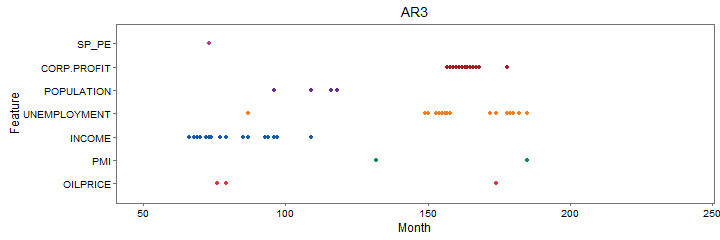
\includegraphics[width=\linewidth]{TimeSeriesAR3.png}
	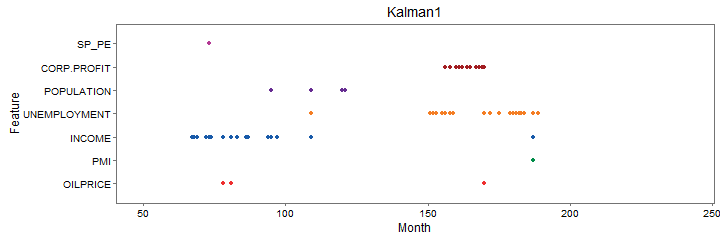
\includegraphics[width=\linewidth]{TimeSeriesKalman1.png}
	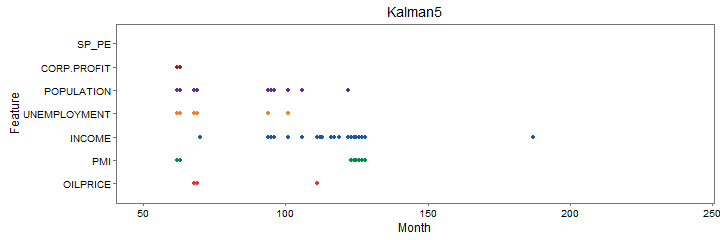
\includegraphics[width=\linewidth]{TimeSeriesKalman5.png}
	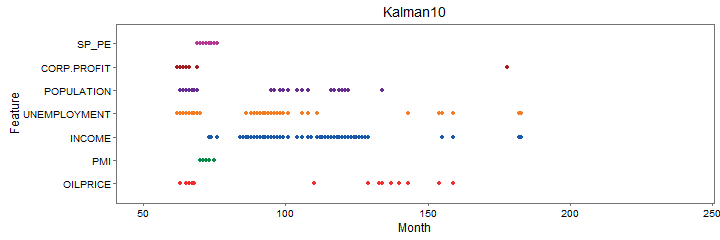
\includegraphics[width=\linewidth]{TimeSeriesKalman10.png}

	\caption{Periods in which each variable is relevant to the sliding window Lasso regularised model for each set of residuals.}
			\label{fig:Window}
\end{figure}

Figure \ref{fig:Window} shows the variables selected by lasso regularisation of each model over time using a sliding window. We see that no variable improves the model all the time with bursts of activity. This makes some intuitive sense as if oil prices are stable it is not likely  to be a strong factor in investors decisions to invest or withdraw from the S\&P. 
We also see that no variables are used through the latter portions of the data. Figure \ref{fig:Residuals} shows that this period in time has much lower residuals, it could be the source of noise of these small residuals are less likely to be directly from econometric data. 
Finally we see many of the same patterns across the different models most prominently the effect of income during the early period and oilprice during specific small bursts of time. 
Table \ref{table:window.results} shows the performance of these predictions overall. We see lower performance than the overall model despite the benefit of locality but this isn't necessarily fair because the sliding window is operating on less data and making unseen predictions whereas the overall data is largely predicting seen data (and validation set). 
\begin{table}[ht]
\centering
\begin{tabular}{llrr}
  \hline
 \textbf{predictors} & \textbf{model} & \textbf{pvalue} & \textbf{rsquared} \\ 
  \hline
  \hline
\multirow{4}{*}{Raw} & Kalman1 & 0.614 & 0.001 \\ 
& Kalman5 & 0.209 & 0.007 \\ 
& Kalman10 & 0.854 & 0.057 \\ 
& AR3 & 0.365 & 0.004 \\ 
  \hline
\multirow{4}{*}{Standardised} & Kalman1 & 0.009 & 0.100 \\ 
& Kalman5 & 0.209 & 0.007 \\ 
& Kalman10 & 0.059 & 0.334 \\ 
& AR3 & 0.365 & 0.004 \\ 
  \hline
\multirow{4}{*}{Kalman} & Kalman1 & 0.616 & 0.001 \\ 
& Kalman5 & 0.209 & 0.007 \\ 
& Kalman10 & 0.912 & 0.053 \\ 
& AR3 & 0.365 & 0.004 \\ 
  \hline
\multirow{4}{*}{Kal \& Std} & Kalman1 & 0.007 & 0.109 \\ 
& Kalman5 & 0.209 & 0.007 \\ 
& Kalman10 & 0.039 & 0.304 \\ 
& AR3 & 0.365 & 0.004 \\ 
   \hline
\end{tabular}
\caption{P values and R squared values for each of 4 models trained on the whole timeseries. In each case lasso regularisation occurs with parameter $\lambda$ trained by minimising mean-squared error through 5-fold cross validation. }
\label{table:fengineering}
\end{table}

\begin{table}[ht]
\centering
\begin{tabular}{lrr}
  \hline
\textbf{model} & \textbf{pvalue} & \textbf{rsquared} \\ 
  \hline
  \hline
Kalman1 & 0.898 & 0.033 \\ 
Kalman5 & 0.479 & 0.087 \\ 
Kalman10 & 0.214 & 0.270 \\ 
AR3 & 0.867 & 0.042 \\ 
  \hline
  \end{tabular}
\caption{P values and R-squareds for predictions trained on a sliding window of previous 50 Months}
\label{table:window.results}
\end{table}


\begin{figure}[ht]
	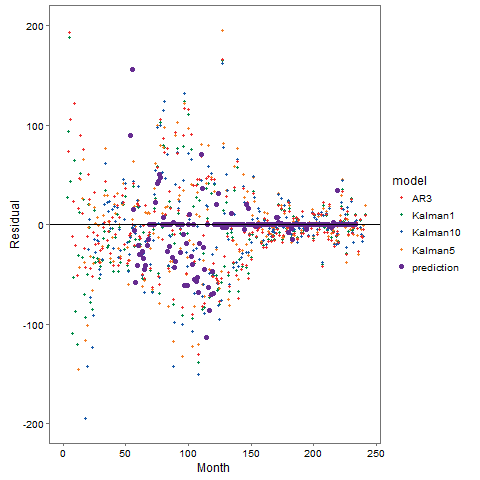
\includegraphics[width=\linewidth]{Residuals.png}
	\centering
	\caption{Size of residuals for each model and prediction of Kalman10 residuals by Lasso regularisation}
			\label{fig:Residuals}
\end{figure}

\begin{figure}[b]
	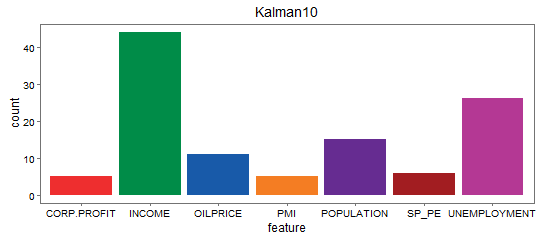
\includegraphics[width=\linewidth]{count_Kalman10.png}
	\centering
	\caption{Number of times that each variable is selected by minimising MSE through lasso regularisation over the sliding window}
			\label{fig:counts}
\end{figure}






\section{Conclusion}
Evaluated on the overall data we found the best performing model was on the residuals of the Kalman10 filter with a p-value of 0.059 and r-squared of 0.33. This is significant enough to say that econometric data can help describe the residuals of state-space models.

However we have seen that the degree to which these variables model the residuals is strongly affected by the order of the Kalman filtering model, with strongest effects given to the weaker models. It is possible the econometric variables are simply capturing variation which was captured by the better performing filter models and lost by the worse ones.  

Evaluated over a sliding we have seen that different variables are active for different periods (often bursts) of time. Further work could be done to assess how predictable the effect of different variables on the model would be. I.e. are there any patterns in the predictor time-series which leads it to be impactful in modelling the residuals at that point. There are periods of time where none of these variables contribute and these periods coincide with smaller model residuals. Overall here p-values are fairly poor but this is likely representative of that the null hypothesis of no relationship is chosen a lot of the time, it is likely that when evaluated only when the model believes it can make a prediction of the residuals p values would be better.  
 
Finally further work can be done in improving the underlying models, either by introducing heteroskedacity modelling via GARCH models, or by introducing mean averaging terms via ARIMA. ARIMA(0,1,1) modelling of stock prices is common in the literature and the distribution of the residuals certainly shows heteroskedacity so it is likely both these methods would improve the models. 
 
\begin{table*}[t]
\centering
\begin{tabular}{rrrr|rrrrrll}
  \hline
model & predictors & rsquared & pvalue & OIL & PMI & INCOME & UNEMP & POP& C.PROFIT & SP\_PE \\ 
  \hline
\multirow{4}{*}{Raw} & Kalman1 & 0.001 & 0.614 & 0.000 & 0.000 & 0.000 & 0.000 & -0.000 & 0.000 & 0.000  \\ 
& Kalman5 & 0.007 & 0.209 & 0.000 & 0.000 & 0.000 & 0.000 & 0.000 & 0.000 & 0.000 \\ 
& Kalman10 & 0.057 & 0.854 & -2.266 & 2.745 & 0.000 & 18.395 & -0.003 & 0.467 & 11.393  \\ 
& AR3 & 0.004 & 0.365 & 0.000 & 0.000 & 0.000 & 0.000 & 0.000 & 0.000 & 0.000  \\ 
\hline
\multirow{4}{*}{Std} & Kalman1 & 0.100 & 0.009 & -3.477 & -1.086 & -48.683 & 4.011 & 59.215 & 1.754 & -6.554 \\ 
& Kalman5 & 0.007 & 0.209 & 0.000 & 0.000 & 0.000 & 0.000 & 0.770 & 0.000 & 0.000  \\ 
& Kalman10 & 0.334 & 0.059 & -15.102 & 21.631 & -1313.228 & 93.629 & 1479.473 & 20.144 & 2.966  \\ 
& AR3 & 0.004 & 0.365 & 0.000 & 0.000 & 0.000 & 0.000 & 0.000 & 0.000 & 0.000  \\ 
\hline
\multirow{4}{*}{Kalman} & Kalman1 & 0.001 & 0.616 & 0.000 & 0.000 & 0.000 & 0.000 & -0.000 & 0.000 & 0.000  \\ 
& Kalman5 & 0.007 & 0.209 & 0.000 & 0.000 & 0.000 & 0.000 & 0.000 & 0.000 & 0.000  \\ 
& Kalman10 & 0.053 & 0.912 & -2.385 & 1.272 & 0.000 & 21.537 & -0.003 & 0.478 & 10.478  \\ 
& AR3 & 0.004 & 0.365 & 0.000 & 0.000 & 0.000 & 0.000 & 0.000 & 0.000 & 0.000   \\ 
\hline
\multirow{4}{*}{Both} & Kalman1 & 0.109 & 0.007 & -2.653 & -0.801 & -60.635 & 4.187 & 69.025 & 3.404 & -5.071  \\ 
& Kalman5 & 0.007 & 0.209 & 0.000 & 0.000 & 0.000 & 0.000 & 0.804 & 0.000 & 0.000 \\ 
& Kalman10 & 0.304 & 0.039 & -8.594 & 10.996 & -1358.679 & 95.975 & 1508.094 & 38.094 & 12.468 \\ 
& AR3 & 0.004 & 0.365 & 0.000 & 0.000 & 0.000 & 0.000 & 0.000 & 0.000 & 0.000   \\ 
   \hline
\end{tabular}
\caption[caption blah]{ Values for weights of each feature chosen for standardised data trained on full time series, by Lasso regularisation model. \footnotemark}
\end{table*}
\footnotetext{AR3 has p values and rsquareds despite no variables being selected due to prediction being against all data but training picking the best of cross validated set}

\bibliographystyle{abbrv}
\bibliography{sigproc}  % sigproc.bib is the name of the 


 
\end{document}